\documentclass[a0, portrait]{IWIposter}

\usepackage{amsmath}
\usepackage{amssymb}
\usepackage{multicol}
\usepackage{graphicx}
\usepackage{epstopdf}
\usepackage{multirow}
\usepackage{tabularx}
\usepackage{graphicx}
\usepackage{xcolor}
\usepackage{url}

\usepackage{mathtools}
\DeclarePairedDelimiter{\abs}{\lvert}{\rvert}

\definecolor{nicepink}{rgb}{0.94, 0.22, 0.81}


\title{A Deep Convolutional Neural Network for Location Recognition and
Geometry Based Information}

\author{\begin{tabular*}{\textwidth}{@{\extracolsep{\fill}} ccccc}
Francesco Bidoia$^{1}$ \hspace{0.5cm} & Matthia Sabatelli$^{1,2}$ \hspace{0.5cm} & Amirhossein Shantia$^{1}$ \hspace{0.5cm} Marco A. Wiering$^{1}$ \hspace{0.5cm} & Lambert Schomaker$^{1}$  \\
%josephgk@hotmail.nl & m.a.wiering@rug.nl & madalina.drugan@gmail.com
\end{tabular*}
}
\institute{$^{1}$Institute of Artificial Intelligence and Cognitive Engineering, University of Groningen \\
	$^{2}$ Montefiore Institute, Department of Electrical Engineering and Computer Science, Universit\'e de Li\`ege, Belgium
}

\DeclareMathOperator{\mean}{E}
\DeclareMathOperator{\var}{Var}
\DeclareMathOperator{\MSE}{MSE}
\DeclareMathOperator{\Cov}{Cov}

\begin{document}

\conference{The 7th International Conference on Pattern Recognition Applications and Methods (ICPRAM)}

\setlength{\columnseprule}{1pt}

\maketitle
	
\begin{multicols}{3}

%===============================================================================

\section*{Introduction}

\begin{itemize}
	\item Autonomous Navigation Systems (ANS) have recently gained a lot of attention from various research domains, nevertheless in order to work well, most of them are based on fairly expensive sensor technologies.
	\item As a solution it is possible to build the ANS based only on visual input (i.e. camera) which, in combination with the odometry of the system, allow the system to map an environment and navigate.
	\item In this work we show that standard Computer Vision and Deep Learning algorithms fail in understanding the visual information that is received as input from a camera. This is given due to their lack in preserving the \textbf{Geometrical Properties} of the images. The consequence of this lack of understanding turns into an ANS which is unable to \textbf{localize} itself.
	\item To solve this problem we present a novel \textbf{Deep Convolutional Neural Network} \cite{szegedy2015going} inspired by the famous \textit{Inception Module} \cite{szegedy2016rethinking} which is tested on $2$ Datasets that we have created: the first one is used for \textit{Scene Recogntion} while the latter one for \textit{Location Recognition}.
\end{itemize}

%===============================================================================

\section*{Datasets Creation}

The Datasets consist in a set of recordings of an environment filled with specifically designed different \textbf{Visual Markers} (VM) as presented in Figure \ref{fig:VisualMarker}. \\

\begin{figure}[H]
	\centering
	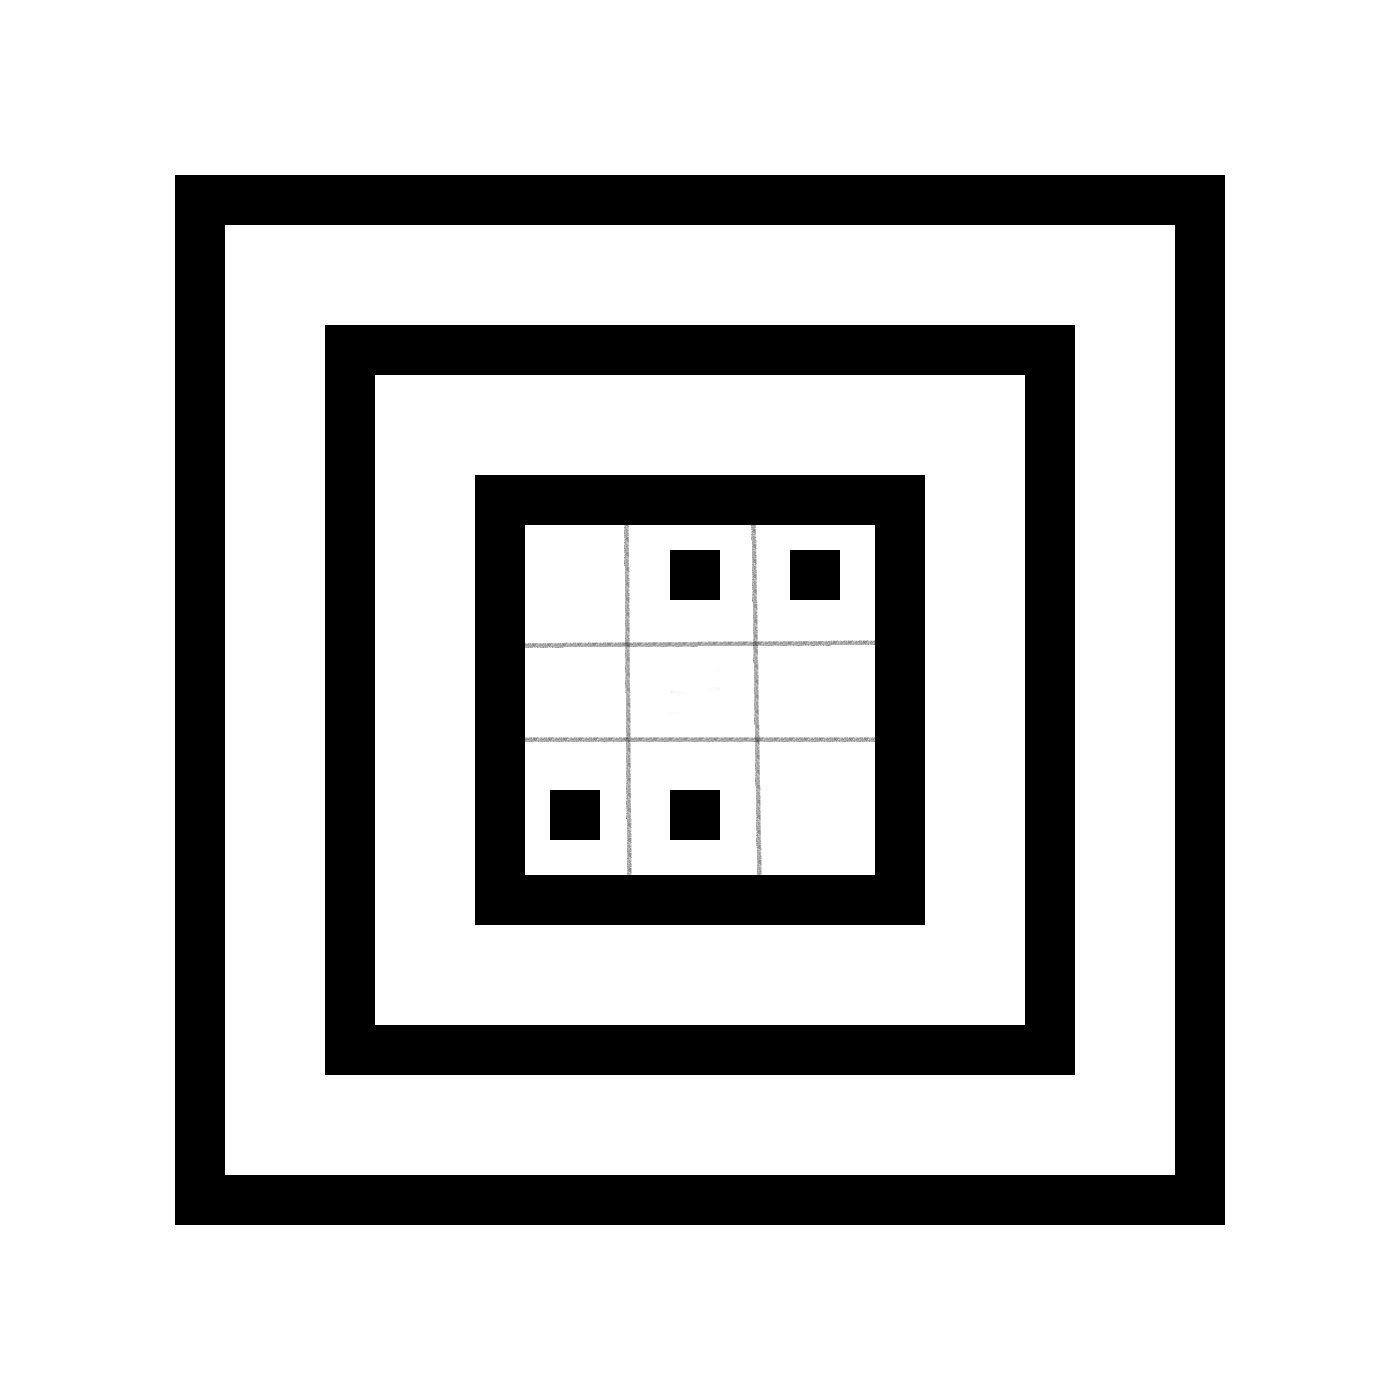
\includegraphics[width=0.5\textwidth]{VisualMarker.png}
	\caption{Example of a Visual Marker used for the creation of the Datasets}
	\label{fig:VisualMarker}
\end{figure}

We assign to each VM, a specific location in the environment which the robot will have to recognize. \\
We create the Datasets as follows:  

\begin{itemize}

\item Scene Recognition Dataset

	\begin{itemize}
	\item $8144$ different pictures
	\item $10$ classes that correspond to $10$ different VMs
	\item Data-Augmentation up to $32,5640$ samples
	\end{itemize}

$80\%$ is used as Training set, while $10\%$ is used as Validation and Testing sets respectively.

\item Location Recognition Dataset

	\begin{itemize}
	\item $1$ Extra class ($\varphi$) is added to the Dataset
	\item $\varphi$ consisting of all the images presented in the previous Dataset but flipped, as shown in Figure \ref{fig:FlippedExamples}
	\end{itemize}

We split the Dataset into $50\%$ for Training and $50\%$ for Testing.
\end{itemize}

\begin{figure}
        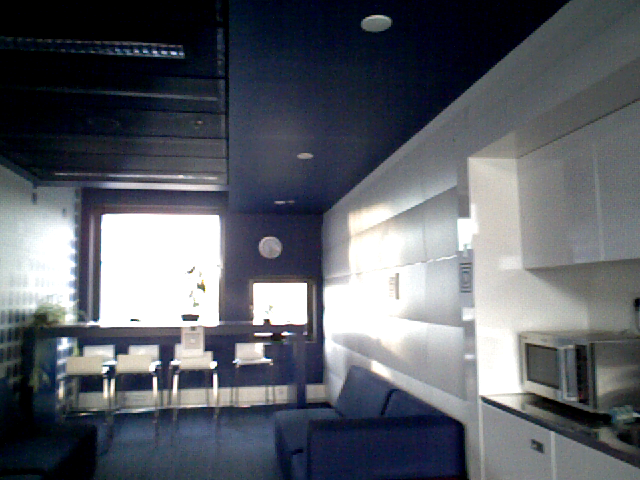
\includegraphics[width=0.475\textwidth]{Position1.png}
        \hfill
        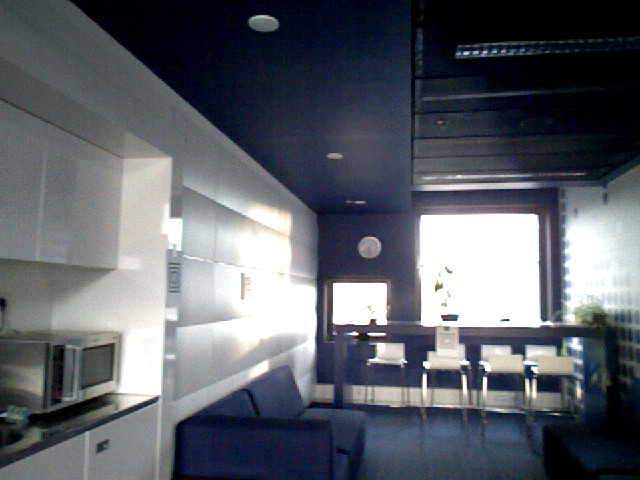
\includegraphics[width=0.475\textwidth]{Position2.png}
	\caption{Two flipped pictures representing the same location. The images have been used as part of the Location Recognition Dataset}
	\label{fig:FlippedExamples}
\end{figure}


%===============================================================================
\section*{Histogram of SIFT Features + Artificial Neural Network}
\begin{itemize}
	\item Proposed by \cite{lowe2004distinctive} the Scale Invariant Feature Transform (SIFT) in combination with the Bag of Visual Word (BOW) was the state of the art technique in Computer Vision before the advent of CNNs
	\item Not suitable for our Dataset which contains pictures with few unique features that do not help the algorithm during the generalization phase
	\item Instead we identify the features via the use of a \textbf{Dense Grid of Key Points} over the images
	as shown in Figure \ref{fig:KeyPoints}

	\begin{figure}[H]
		\centering
		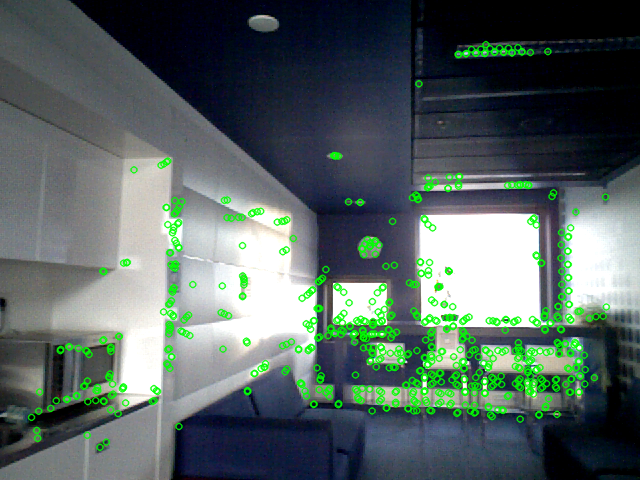
\includegraphics[width=0.5\textwidth]{key.png}
		\caption{Visualization of the Key Points on an Image present in the Datasets}
		\label{fig:KeyPoints}
	\end{figure}
	
	\item We obtain:
	\begin{itemize}
		\item $1$ key point every $8$ pixels
		\item Total of $5440$ key points per picture
		\item $128$ features long vector per key point
	\end{itemize}

	\item We use the BOW clustering algorithm to reduce the amount of features which are then given to an Artificial Neural Network for the final classification 

\end{itemize}

%===============================================================================

\section*{Inception V3 Convolutional Neural Network}

This Artificial Neural Network consists in:

\begin{itemize}

	\item $33$ layers deep neural network
	\item Replaces $5 \times 5$ convolutions with two consecutive $3 \times 3$ ones as shown in Figure \ref{fig:ConvolutionsExample}
	\item Similarly a $3 \times 3$ convolution is replaced by $3 \times 1$ and $1 \times 3$ convolutions
	\item We take the original architecture publicly available on \verb#GitHub# \footnote{
\url{https://github.com/tensorflow/models/tree/master/inception}} and train only a final fully connected layer of $250$ hidden units
	\item $\approx 1.3$ million of parameters have to be trained
	\item Due to the extensive use of \textbf{Pooling} the geometrical properties of the inputs get changed misleading the \textbf{Localization} phase

\end{itemize}

\begin{figure}[H]
	\centering
	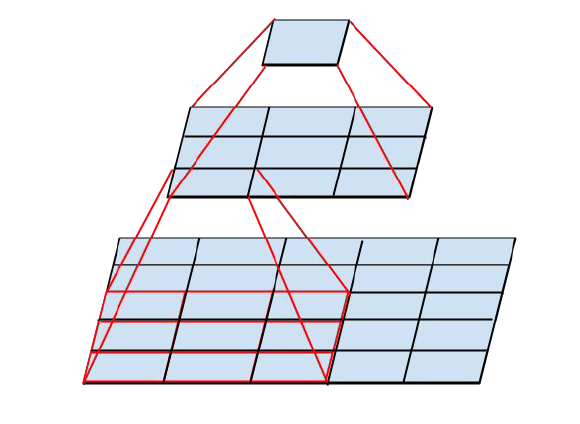
\includegraphics[width=0.5\textwidth]{ConvolutionsExample.png}
	\caption{Example of how two $3 \times 3$ convolutions can be used instead of a $5 \times 5$ one}
	\label{fig:ConvolutionsExample}
\end{figure}


%===============================================================================

\section*{Novel Deep Convolutional Neural Network Architecture}

We propose the following neural architecture.

\centering
\subsubsection*{Motivation}
	\begin{itemize}
		\item Use the optimization techniques of the Inception $V3$ architecture presented in Figure \ref{fig:ConvolutionsExample}
		\item \textbf{Avoid Pooling} in order to preserve the geometrical information of the input

	\end{itemize}

\centering
\subsubsection*{Neural Architecture}
	\begin{itemize}
		\item Input Images as a $300 \times 300 \times 3$ tensor
		\item $7 \times 7$ convolution with $48$ channels and strides $= 3$
		\item $9 \times 9$ convolution with $32$ channels and strides $= 2$ 
		\item $11 \times 11$ convolution with $24$ channels and strides $= 1$ 
		\item $22 \times 22$ convolution with $16$ channels and strides $= 1$ 
		\item \textbf{Inception Module} that uses a $1 \times 1$ followed by a $3 \times 3$ convolution in parallel with a $1 \times 1$ and $5 \times 5$ one
		\item Final fully connected layer of $200$ Hidden Units
		\item \textit{Rectified Linear Unit} (ReLU) $f(x) = max(0,x)$ as activation function
		\item Dropout rate of $0.1$

	\end{itemize}


%===============================================================================
\section*{Results}

\centering
\subsubsection*{Scene Dataset Accuracies}

\begin{itemize}
	\item We report in Table \ref{tab:tab1} the accuracies that have been obtained by the different Computer Vision algorithms. $\tau$ refers to the amount of computation time in hours.
\end{itemize}

\begin{table}
\centering
\caption{The accuracies on the Scene Dataset}
\label{tab:tab1}
\begin{tabular}{>{\rowmac}l|>{\rowmac}l|>{\rowmac}l|>{\rowmac}l<{\clearrow}}
\textbf{Algorithm}   & \textbf{Validation-Set} & \textbf{Testing-Set} & \textbf{$\tau$}  \\ \hline
        BOW                    & $89.7\%$             & $88.5\%$           & $72$    \\
        Inception $V3$         & $100\%$              & $100\%$            & $2.3$     \\
        DCNN                   & $100\%$              & $98.7\%$           & $1.5$          \\
\end{tabular}\label{tab:tab1}
\end{table}

\begin{itemize}
	\item Despite being the architecture performing best we see that the Inception $V3$ does not generalize when tested on the Location Dataset.
	\item We report in Table \ref{tab:tab2} the accuracies of the neural architectures. We introduce the class \textbf{Tricked} in which we report if the ANN labels a flipped image as an original one.
\end{itemize}

\centering
\subsubsection*{Location Dataset Accuracies}

\begin{table}
\centering
\caption{The accuracies on the Location Dataset}
\begin{tabular}{>{\rowmac}l|>{\rowmac}l|>{\rowmac}l|>{\rowmac}l<{\clearrow}}
\textbf{Algorithm}   & \textbf{Correct} & \textbf{Tricked} & \textbf{Missed}  \\ \hline
       Inception $V3$         & $0\%$              & $97.43\%$            & $2.57\%$     \\
       DCNN                   & $99.7\%$              & $0\%$           & $0.3\%$          \\
\end{tabular}\label{tab:tab2}
\end{table}

\begin{itemize}
	\item We see that our novel DCNN is able to classify correctly the images in the Location Dataset, meaning that the geometrical properties of the input are maintained. 
	\item Figure \ref{fig:SoftmaxOutput} shows the robustness of the system that makes use of our neural architecture in a simulated environment. 
\end{itemize}


\begin{figure}
        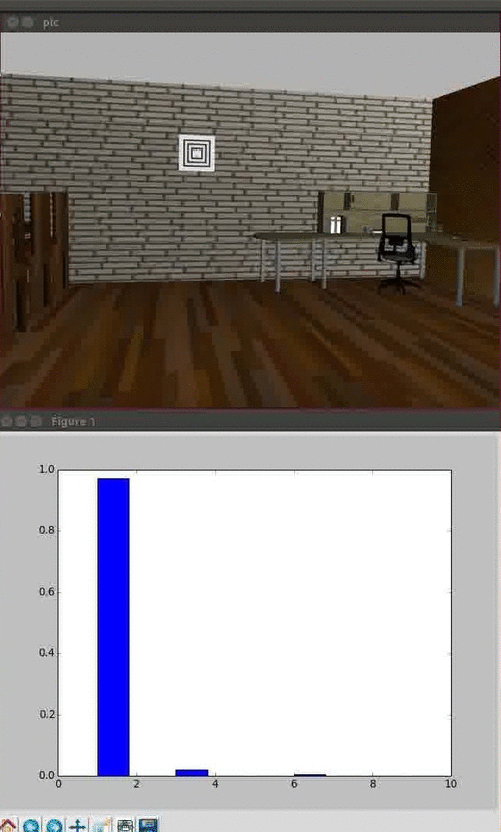
\includegraphics[width=0.275\textwidth]{position1.png}
        \hfill
        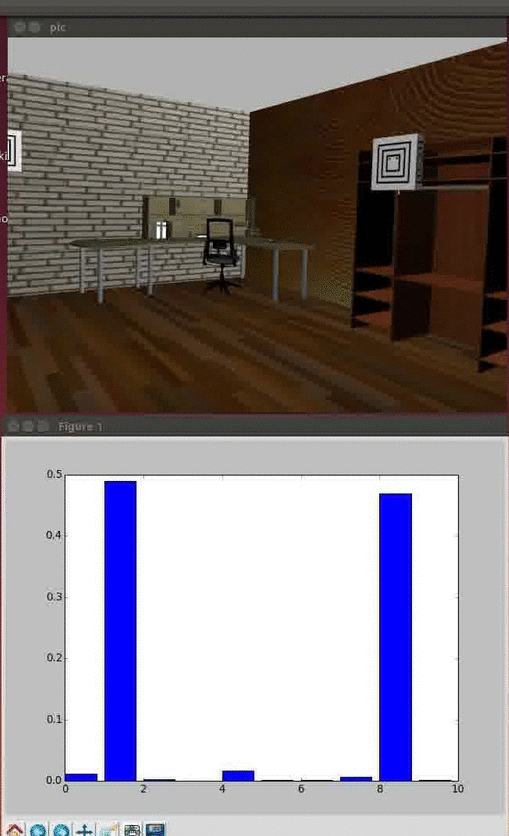
\includegraphics[width=0.275\textwidth]{position2.png}
	\hfill
	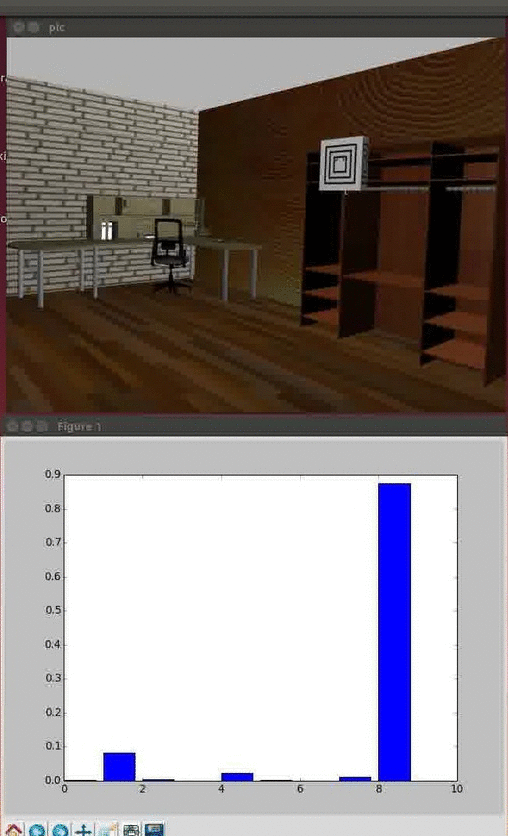
\includegraphics[width=0.275\textwidth]{position3.png}
	\caption{The softmax output of the DCNN on two flipped pictures representing the same location. We observe how the ANN is able to distinguish the two locations}
	\label{fig:SoftmaxOutput}
\end{figure}



%===============================================================================
\section*{Conclusion}

\begin{itemize}
	\item In this work we show how it is possible to build Deep Convolutional Neural Networks without having to rely on dimensionality reduction techniques such as \textbf{Pooling}.
	\item We show how this can be particularly useful in the context of Autonomous Navigation Systems that are based on visual input. 

\end{itemize}


\bibliographystyle{plain}
\bibliography{mybibfile}
\end{multicols}

\end{document}
